\documentclass[twoside,UTF8]{EPURapport}
\usepackage[utf8]{inputenc}
%\usepackage{listings}

%\renewcommand{\lstlistlistingname}{Liste des codes}
%\renewcommand{\lstlistingname}{Code}

%\addextratables{%
%	\lstlistoflistings
%}

%\swapAuthorsAndSupervisors

%\RequirePackage{colortbl}

\usepackage{tikz}

\thedocument{Rapport de mini-projet}{Automaton Cellular}{Automaton Cellular}

\grade{Département Informatique\\ 4\ieme{} année\\ 2011 - 2012}

\authors{%
	\category{Étudiants}{%
		\name{Abdelnor BOUSMINA} \mail{abdelnor.bousmina@etu.univ-tours.fr}
		\name{Albin POIGNOT} \mail{albin.poignot@etu.univ-tours.fr}
	}
	\details{DI4 2011 - 2012}
}

\supervisors{%
	\category{Encadrants}{%
		\name{Emmanuel NERON} \mail{emmanuel.neron@univ-tours.fr}
	}
	\details{Université François-Rabelais, Tours}
}

\abstracts{Implémentation d'un modèle mathématique simulant l'évacuation de piétons d'une salle. Elle génère également des diagrammes représentant certaines statistiques sur le déroulement de l'évacuation.}
{java, évacuation, modèle mathématique, automate cellulaire}
{Description en anglais}
{java, evacuation, mathematic model, automaton cellular}

\begin{document}

\chapter{Introduction}
	\section{Objectifs du projet}
	Ce projet a pour objectif d'implémenter un modèle mathématique fourni. Ce dernier simule le déplacement de piétons. Dans notre cas, nous voulons utiliser ce modèle pour simuler l'évacuation d'une salle remplie de personnes. L'application fournie également des diagrammes représentant le temps écoulé avant évacuation de la dernière personne ainsi que la distance parcourue.\\
	Incluant certains facteurs aléatoires comme l'état de panique et la gestion des "collisions", de telles données vont permettre d'analyser l'influence des comportements imprévisibles des personnes lors d'une évacuation d'urgence.
	
\chapter{Méthodes et résultats}

	\section{Modèle mathématique}
	Le modèle mathématique utilisé a été présenté dans un papier écrit par A. Varasa, M.D. Cornejoa, D. Mainemera, B. Toledob, J. Rogana, V. Munoza et J.A. Valdiviaa. \\
	Ce modèle représente une pièce comme une grille 2D. Chaque case de cette grille pouvant être vide, occupée par une personne ou par un obstacle. On considère que chaque case représente un espace de $0,4 * 0,4 m^2$ dans le monde réel. Cette surface est celle typiquement occupée par une personne dans une foule dense. Ainsi, en considérant une vitesse de marche moyenne de $1m/s$, lorsqu'une personne bouge de $0,4m$, on a donc $\Delta t \approx 0.4$.\\
	Ensuite, les mouvements des personnes sont déterminé par (1) un plan fixe de la configuration de la salle, calculé de façon à ce que la case la plus proche de la sortie soit préférée, et par (2) l'interaction entre les personnes.
	
	\subsection{La configuration de la salle}
	A la création du système, la taille de la pièce ainsi que la position de la sortie sont déterminées. En sachant cela, une valeur est assignée à chaque case, représentant sa distance à la porte : au plus la valeur est faible, au plus la case est proche de la sortie. C'est à partir de cette configuration statique que les personnes auront la possibilité de déterminer la prochaine case à rejoindre : celle qui a une valeur plus faible que là où il se trouve actuellement. \\
	L'algorithme utilisé est très clairement décrit dans le papier :
	\begin{enumerate}
	\item La pièce est divisée en une grille rectangulaire. La porte de sortie a une valeur de 1.
	\item Ensuite, toutes les cellules adjacente à la précédente (un second ``layer'' de cellules) se voient assigner des valeurs de la façon suivante :
		\begin{enumerate}
			\item Si une cellule a une valeur $N$, alors la cellule adjacente dans les directions verticales et horizontales ont une valeur $N + 1$. Nous allons permettre les déplacements en diagonale, donc il est pertinent de considérer les cellules en diagonale. On leur assigne alors une valeur $N + \lambda$ avec $\lambda \sup 1$. Nous faisons cela dans le but de représenter le fait que la distance entre deux cases diagonalement est plus grande que celle entre deux cases horizontalement ou verticalement adjacentes. (Le papier a choisi une valeur arbitraire de $\lambda = 3$. Dans notre projet, la valeur est personalisable).
			\item Si il y a un conflit lors d'une assignation de valeur, alors la valeur minimum est assignée.
		\end{enumerate}

		\item Puis le troisième ``layer'' de cellules est calculé, composé de toutes les cellules adjacentes à celle du second, mais pas celle du premier.
		\item Le processus est répété jusqu'à ce que toutes les cellules soient évaluées.
		\item Les murs sont également considérés lors de la définition de la grille. Les cellules représentant les murs ont des valeurs très élevées. Cela assurera que les personnes ne choisiront jamais de se placer sur ces cellules. (Les obstacles seront donc gérés de la même façon).
	\end{enumerate}

	
	\section{Solutions techniques}
	Pour la réalisation de ce projet, nous avons choisi d'utiliser le langage Java. De plus, pour la gestion des diagrammes, nous avons également utilisé une librairie dédiée à cette tâche : JFreeChart. De façon à structurer les sources, nous avons mis en place une structure MVC (Model-View-Controler). Cette façon de programmer permet de séparer les différents modules en les rendant les plus indépendants possibles les uns des autres. Cela améliore la maintenabilité ainsi que la réutilisabilité du code.\\
	En suivant cette méthode, voici comment nous avons organisé nos sources :
	
	\begin{enumerate}
		\item Package "Controlleur"
		\begin{itemize}
			\item \textbf{Controller} : organise les interactions entre les classes du package Modele elle-même mais aussi entre les classes du package Modele et du package Vue
		\end{itemize}
		
		\item Package "Modele"
		\begin{itemize}
			\item \textbf{Grille} : chargée de gérer la génération de la grille et de ses obstacles
			\item \textbf{MathModel} : implémentation du modèle mathématique : fourni la prochaine position d'une personne
			\item \textbf{Neighborhood} : fourni les cases voisines d'une personne
			\item \textbf{Obstacle} : représente un obstacle
			\item \textbf{Person} : représente une personne
		\end{itemize}
		
		\item Package "Vue"
		\begin{itemize}
			\item \textbf{Chart} : dessine un diagramme en batons
			\item \textbf{ChartLine} : dessine un diagramme dessinant une courbe
			\item \textbf{DrawAreaUI} : aire de dessin des composants de l'application
			\item \textbf{GrilleUI} : représente la partie graphique d'une instance de Grille 
			\item \textbf{MainWindow} : fenêtre principale (contient la fonction main())
			\item \textbf{PersonUI} : représente la partie graphique d'une instance de Personne
		\end{itemize}
	\end{enumerate}	
	
	Le schéma UML suivant fourni une vision globale des classes implémentées : ~\ref{fig:uml}\\
	
%	% Graphic for TeX using PGF
% Title: /home/albin/Developpements/EclipseWorkspace/Automaton-Cellular/UML.dia
% Creator: Dia v0.97.2
% CreationDate: Fri May 18 21:42:13 2012
% For: albin
% \usepackage{tikz}
% The following commands are not supported in PSTricks at present
% We define them conditionally, so when they are implemented,
% this pgf file will use them.
\ifx\du\undefined
  \newlength{\du}
\fi
\setlength{\du}{15\unitlength}
\begin{tikzpicture}
\pgftransformxscale{1.000000}
\pgftransformyscale{-1.000000}
\definecolor{dialinecolor}{rgb}{0.000000, 0.000000, 0.000000}
\pgfsetstrokecolor{dialinecolor}
\definecolor{dialinecolor}{rgb}{1.000000, 1.000000, 1.000000}
\pgfsetfillcolor{dialinecolor}
\pgfsetlinewidth{0.100000\du}
\pgfsetdash{}{0pt}
\definecolor{dialinecolor}{rgb}{1.000000, 1.000000, 1.000000}
\pgfsetfillcolor{dialinecolor}
\fill (1.400000\du,1.900000\du)--(1.400000\du,10.800000\du)--(14.450000\du,10.800000\du)--(14.450000\du,1.900000\du)--cycle;
\definecolor{dialinecolor}{rgb}{0.000000, 0.000000, 0.000000}
\pgfsetstrokecolor{dialinecolor}
\draw (1.400000\du,1.900000\du)--(1.400000\du,10.800000\du)--(14.450000\du,10.800000\du)--(14.450000\du,1.900000\du)--cycle;
\definecolor{dialinecolor}{rgb}{1.000000, 1.000000, 1.000000}
\pgfsetfillcolor{dialinecolor}
\fill (1.400000\du,0.900000\du)--(1.400000\du,1.900000\du)--(3.525000\du,1.900000\du)--(3.525000\du,0.900000\du)--cycle;
\definecolor{dialinecolor}{rgb}{0.000000, 0.000000, 0.000000}
\pgfsetstrokecolor{dialinecolor}
\draw (1.400000\du,0.900000\du)--(1.400000\du,1.900000\du)--(3.525000\du,1.900000\du)--(3.525000\du,0.900000\du)--cycle;
% setfont left to latex
\definecolor{dialinecolor}{rgb}{0.000000, 0.000000, 0.000000}
\pgfsetstrokecolor{dialinecolor}
\node[anchor=west] at (1.500000\du,1.650000\du){Model};
\pgfsetlinewidth{0.100000\du}
\pgfsetdash{}{0pt}
\definecolor{dialinecolor}{rgb}{1.000000, 1.000000, 1.000000}
\pgfsetfillcolor{dialinecolor}
\fill (1.750000\du,2.400000\du)--(1.750000\du,3.800000\du)--(7.272500\du,3.800000\du)--(7.272500\du,2.400000\du)--cycle;
\definecolor{dialinecolor}{rgb}{0.000000, 0.000000, 0.000000}
\pgfsetstrokecolor{dialinecolor}
\draw (1.750000\du,2.400000\du)--(1.750000\du,3.800000\du)--(7.272500\du,3.800000\du)--(7.272500\du,2.400000\du)--cycle;
% setfont left to latex
\definecolor{dialinecolor}{rgb}{0.000000, 0.000000, 0.000000}
\pgfsetstrokecolor{dialinecolor}
\node at (4.511250\du,3.350000\du){MathModel};
\definecolor{dialinecolor}{rgb}{1.000000, 1.000000, 1.000000}
\pgfsetfillcolor{dialinecolor}
\fill (1.750000\du,3.800000\du)--(1.750000\du,4.200000\du)--(7.272500\du,4.200000\du)--(7.272500\du,3.800000\du)--cycle;
\definecolor{dialinecolor}{rgb}{0.000000, 0.000000, 0.000000}
\pgfsetstrokecolor{dialinecolor}
\draw (1.750000\du,3.800000\du)--(1.750000\du,4.200000\du)--(7.272500\du,4.200000\du)--(7.272500\du,3.800000\du)--cycle;
\definecolor{dialinecolor}{rgb}{1.000000, 1.000000, 1.000000}
\pgfsetfillcolor{dialinecolor}
\fill (1.750000\du,4.200000\du)--(1.750000\du,4.600000\du)--(7.272500\du,4.600000\du)--(7.272500\du,4.200000\du)--cycle;
\definecolor{dialinecolor}{rgb}{0.000000, 0.000000, 0.000000}
\pgfsetstrokecolor{dialinecolor}
\draw (1.750000\du,4.200000\du)--(1.750000\du,4.600000\du)--(7.272500\du,4.600000\du)--(7.272500\du,4.200000\du)--cycle;
\pgfsetlinewidth{0.100000\du}
\pgfsetdash{}{0pt}
\definecolor{dialinecolor}{rgb}{1.000000, 1.000000, 1.000000}
\pgfsetfillcolor{dialinecolor}
\fill (1.780000\du,5.025000\du)--(1.780000\du,6.425000\du)--(8.670000\du,6.425000\du)--(8.670000\du,5.025000\du)--cycle;
\definecolor{dialinecolor}{rgb}{0.000000, 0.000000, 0.000000}
\pgfsetstrokecolor{dialinecolor}
\draw (1.780000\du,5.025000\du)--(1.780000\du,6.425000\du)--(8.670000\du,6.425000\du)--(8.670000\du,5.025000\du)--cycle;
% setfont left to latex
\definecolor{dialinecolor}{rgb}{0.000000, 0.000000, 0.000000}
\pgfsetstrokecolor{dialinecolor}
\node at (5.225000\du,5.975000\du){Neighborhood};
\definecolor{dialinecolor}{rgb}{1.000000, 1.000000, 1.000000}
\pgfsetfillcolor{dialinecolor}
\fill (1.780000\du,6.425000\du)--(1.780000\du,6.825000\du)--(8.670000\du,6.825000\du)--(8.670000\du,6.425000\du)--cycle;
\definecolor{dialinecolor}{rgb}{0.000000, 0.000000, 0.000000}
\pgfsetstrokecolor{dialinecolor}
\draw (1.780000\du,6.425000\du)--(1.780000\du,6.825000\du)--(8.670000\du,6.825000\du)--(8.670000\du,6.425000\du)--cycle;
\definecolor{dialinecolor}{rgb}{1.000000, 1.000000, 1.000000}
\pgfsetfillcolor{dialinecolor}
\fill (1.780000\du,6.825000\du)--(1.780000\du,7.225000\du)--(8.670000\du,7.225000\du)--(8.670000\du,6.825000\du)--cycle;
\definecolor{dialinecolor}{rgb}{0.000000, 0.000000, 0.000000}
\pgfsetstrokecolor{dialinecolor}
\draw (1.780000\du,6.825000\du)--(1.780000\du,7.225000\du)--(8.670000\du,7.225000\du)--(8.670000\du,6.825000\du)--cycle;
\pgfsetlinewidth{0.100000\du}
\pgfsetdash{}{0pt}
\definecolor{dialinecolor}{rgb}{1.000000, 1.000000, 1.000000}
\pgfsetfillcolor{dialinecolor}
\fill (11.160000\du,7.850000\du)--(11.160000\du,9.250000\du)--(13.560000\du,9.250000\du)--(13.560000\du,7.850000\du)--cycle;
\definecolor{dialinecolor}{rgb}{0.000000, 0.000000, 0.000000}
\pgfsetstrokecolor{dialinecolor}
\draw (11.160000\du,7.850000\du)--(11.160000\du,9.250000\du)--(13.560000\du,9.250000\du)--(13.560000\du,7.850000\du)--cycle;
% setfont left to latex
\definecolor{dialinecolor}{rgb}{0.000000, 0.000000, 0.000000}
\pgfsetstrokecolor{dialinecolor}
\node at (12.360000\du,8.800000\du){Grid};
\definecolor{dialinecolor}{rgb}{1.000000, 1.000000, 1.000000}
\pgfsetfillcolor{dialinecolor}
\fill (11.160000\du,9.250000\du)--(11.160000\du,9.650000\du)--(13.560000\du,9.650000\du)--(13.560000\du,9.250000\du)--cycle;
\definecolor{dialinecolor}{rgb}{0.000000, 0.000000, 0.000000}
\pgfsetstrokecolor{dialinecolor}
\draw (11.160000\du,9.250000\du)--(11.160000\du,9.650000\du)--(13.560000\du,9.650000\du)--(13.560000\du,9.250000\du)--cycle;
\definecolor{dialinecolor}{rgb}{1.000000, 1.000000, 1.000000}
\pgfsetfillcolor{dialinecolor}
\fill (11.160000\du,9.650000\du)--(11.160000\du,10.050000\du)--(13.560000\du,10.050000\du)--(13.560000\du,9.650000\du)--cycle;
\definecolor{dialinecolor}{rgb}{0.000000, 0.000000, 0.000000}
\pgfsetstrokecolor{dialinecolor}
\draw (11.160000\du,9.650000\du)--(11.160000\du,10.050000\du)--(13.560000\du,10.050000\du)--(13.560000\du,9.650000\du)--cycle;
\pgfsetlinewidth{0.100000\du}
\pgfsetdash{}{0pt}
\definecolor{dialinecolor}{rgb}{1.000000, 1.000000, 1.000000}
\pgfsetfillcolor{dialinecolor}
\fill (1.790000\du,7.725000\du)--(1.790000\du,9.125000\du)--(6.232500\du,9.125000\du)--(6.232500\du,7.725000\du)--cycle;
\definecolor{dialinecolor}{rgb}{0.000000, 0.000000, 0.000000}
\pgfsetstrokecolor{dialinecolor}
\draw (1.790000\du,7.725000\du)--(1.790000\du,9.125000\du)--(6.232500\du,9.125000\du)--(6.232500\du,7.725000\du)--cycle;
% setfont left to latex
\definecolor{dialinecolor}{rgb}{0.000000, 0.000000, 0.000000}
\pgfsetstrokecolor{dialinecolor}
\node at (4.011250\du,8.675000\du){Obstacle};
\definecolor{dialinecolor}{rgb}{1.000000, 1.000000, 1.000000}
\pgfsetfillcolor{dialinecolor}
\fill (1.790000\du,9.125000\du)--(1.790000\du,9.525000\du)--(6.232500\du,9.525000\du)--(6.232500\du,9.125000\du)--cycle;
\definecolor{dialinecolor}{rgb}{0.000000, 0.000000, 0.000000}
\pgfsetstrokecolor{dialinecolor}
\draw (1.790000\du,9.125000\du)--(1.790000\du,9.525000\du)--(6.232500\du,9.525000\du)--(6.232500\du,9.125000\du)--cycle;
\definecolor{dialinecolor}{rgb}{1.000000, 1.000000, 1.000000}
\pgfsetfillcolor{dialinecolor}
\fill (1.790000\du,9.525000\du)--(1.790000\du,9.925000\du)--(6.232500\du,9.925000\du)--(6.232500\du,9.525000\du)--cycle;
\definecolor{dialinecolor}{rgb}{0.000000, 0.000000, 0.000000}
\pgfsetstrokecolor{dialinecolor}
\draw (1.790000\du,9.525000\du)--(1.790000\du,9.925000\du)--(6.232500\du,9.925000\du)--(6.232500\du,9.525000\du)--cycle;
\pgfsetlinewidth{0.100000\du}
\pgfsetdash{}{0pt}
\definecolor{dialinecolor}{rgb}{1.000000, 1.000000, 1.000000}
\pgfsetfillcolor{dialinecolor}
\fill (9.970000\du,2.350000\du)--(9.970000\du,3.750000\du)--(13.590000\du,3.750000\du)--(13.590000\du,2.350000\du)--cycle;
\definecolor{dialinecolor}{rgb}{0.000000, 0.000000, 0.000000}
\pgfsetstrokecolor{dialinecolor}
\draw (9.970000\du,2.350000\du)--(9.970000\du,3.750000\du)--(13.590000\du,3.750000\du)--(13.590000\du,2.350000\du)--cycle;
% setfont left to latex
\definecolor{dialinecolor}{rgb}{0.000000, 0.000000, 0.000000}
\pgfsetstrokecolor{dialinecolor}
\node at (11.780000\du,3.300000\du){Person};
\definecolor{dialinecolor}{rgb}{1.000000, 1.000000, 1.000000}
\pgfsetfillcolor{dialinecolor}
\fill (9.970000\du,3.750000\du)--(9.970000\du,4.150000\du)--(13.590000\du,4.150000\du)--(13.590000\du,3.750000\du)--cycle;
\definecolor{dialinecolor}{rgb}{0.000000, 0.000000, 0.000000}
\pgfsetstrokecolor{dialinecolor}
\draw (9.970000\du,3.750000\du)--(9.970000\du,4.150000\du)--(13.590000\du,4.150000\du)--(13.590000\du,3.750000\du)--cycle;
\definecolor{dialinecolor}{rgb}{1.000000, 1.000000, 1.000000}
\pgfsetfillcolor{dialinecolor}
\fill (9.970000\du,4.150000\du)--(9.970000\du,4.550000\du)--(13.590000\du,4.550000\du)--(13.590000\du,4.150000\du)--cycle;
\definecolor{dialinecolor}{rgb}{0.000000, 0.000000, 0.000000}
\pgfsetstrokecolor{dialinecolor}
\draw (9.970000\du,4.150000\du)--(9.970000\du,4.550000\du)--(13.590000\du,4.550000\du)--(13.590000\du,4.150000\du)--cycle;
\pgfsetlinewidth{0.100000\du}
\pgfsetdash{}{0pt}
\definecolor{dialinecolor}{rgb}{1.000000, 1.000000, 1.000000}
\pgfsetfillcolor{dialinecolor}
\fill (1.450000\du,12.650000\du)--(1.450000\du,16.150000\du)--(9.700000\du,16.150000\du)--(9.700000\du,12.650000\du)--cycle;
\definecolor{dialinecolor}{rgb}{0.000000, 0.000000, 0.000000}
\pgfsetstrokecolor{dialinecolor}
\draw (1.450000\du,12.650000\du)--(1.450000\du,16.150000\du)--(9.700000\du,16.150000\du)--(9.700000\du,12.650000\du)--cycle;
\definecolor{dialinecolor}{rgb}{1.000000, 1.000000, 1.000000}
\pgfsetfillcolor{dialinecolor}
\fill (1.450000\du,11.650000\du)--(1.450000\du,12.650000\du)--(5.500000\du,12.650000\du)--(5.500000\du,11.650000\du)--cycle;
\definecolor{dialinecolor}{rgb}{0.000000, 0.000000, 0.000000}
\pgfsetstrokecolor{dialinecolor}
\draw (1.450000\du,11.650000\du)--(1.450000\du,12.650000\du)--(5.500000\du,12.650000\du)--(5.500000\du,11.650000\du)--cycle;
% setfont left to latex
\definecolor{dialinecolor}{rgb}{0.000000, 0.000000, 0.000000}
\pgfsetstrokecolor{dialinecolor}
\node[anchor=west] at (1.550000\du,12.400000\du){Controller};
\pgfsetlinewidth{0.100000\du}
\pgfsetdash{}{0pt}
\definecolor{dialinecolor}{rgb}{1.000000, 1.000000, 1.000000}
\pgfsetfillcolor{dialinecolor}
\fill (3.100000\du,13.350000\du)--(3.100000\du,14.750000\du)--(8.122500\du,14.750000\du)--(8.122500\du,13.350000\du)--cycle;
\definecolor{dialinecolor}{rgb}{0.000000, 0.000000, 0.000000}
\pgfsetstrokecolor{dialinecolor}
\draw (3.100000\du,13.350000\du)--(3.100000\du,14.750000\du)--(8.122500\du,14.750000\du)--(8.122500\du,13.350000\du)--cycle;
% setfont left to latex
\definecolor{dialinecolor}{rgb}{0.000000, 0.000000, 0.000000}
\pgfsetstrokecolor{dialinecolor}
\node at (5.611250\du,14.300000\du){Controller};
\definecolor{dialinecolor}{rgb}{1.000000, 1.000000, 1.000000}
\pgfsetfillcolor{dialinecolor}
\fill (3.100000\du,14.750000\du)--(3.100000\du,15.150000\du)--(8.122500\du,15.150000\du)--(8.122500\du,14.750000\du)--cycle;
\definecolor{dialinecolor}{rgb}{0.000000, 0.000000, 0.000000}
\pgfsetstrokecolor{dialinecolor}
\draw (3.100000\du,14.750000\du)--(3.100000\du,15.150000\du)--(8.122500\du,15.150000\du)--(8.122500\du,14.750000\du)--cycle;
\definecolor{dialinecolor}{rgb}{1.000000, 1.000000, 1.000000}
\pgfsetfillcolor{dialinecolor}
\fill (3.100000\du,15.150000\du)--(3.100000\du,15.550000\du)--(8.122500\du,15.550000\du)--(8.122500\du,15.150000\du)--cycle;
\definecolor{dialinecolor}{rgb}{0.000000, 0.000000, 0.000000}
\pgfsetstrokecolor{dialinecolor}
\draw (3.100000\du,15.150000\du)--(3.100000\du,15.550000\du)--(8.122500\du,15.550000\du)--(8.122500\du,15.150000\du)--cycle;
\pgfsetlinewidth{0.100000\du}
\pgfsetdash{}{0pt}
\definecolor{dialinecolor}{rgb}{1.000000, 1.000000, 1.000000}
\pgfsetfillcolor{dialinecolor}
\fill (15.350000\du,1.750000\du)--(15.350000\du,10.850000\du)--(31.600000\du,10.850000\du)--(31.600000\du,1.750000\du)--cycle;
\definecolor{dialinecolor}{rgb}{0.000000, 0.000000, 0.000000}
\pgfsetstrokecolor{dialinecolor}
\draw (15.350000\du,1.750000\du)--(15.350000\du,10.850000\du)--(31.600000\du,10.850000\du)--(31.600000\du,1.750000\du)--cycle;
\definecolor{dialinecolor}{rgb}{1.000000, 1.000000, 1.000000}
\pgfsetfillcolor{dialinecolor}
\fill (15.350000\du,0.750000\du)--(15.350000\du,1.750000\du)--(17.350000\du,1.750000\du)--(17.350000\du,0.750000\du)--cycle;
\definecolor{dialinecolor}{rgb}{0.000000, 0.000000, 0.000000}
\pgfsetstrokecolor{dialinecolor}
\draw (15.350000\du,0.750000\du)--(15.350000\du,1.750000\du)--(17.350000\du,1.750000\du)--(17.350000\du,0.750000\du)--cycle;
% setfont left to latex
\definecolor{dialinecolor}{rgb}{0.000000, 0.000000, 0.000000}
\pgfsetstrokecolor{dialinecolor}
\node[anchor=west] at (15.450000\du,1.500000\du){View};
\pgfsetlinewidth{0.100000\du}
\pgfsetdash{}{0pt}
\definecolor{dialinecolor}{rgb}{1.000000, 1.000000, 1.000000}
\pgfsetfillcolor{dialinecolor}
\fill (15.950000\du,7.800000\du)--(15.950000\du,9.200000\du)--(19.297500\du,9.200000\du)--(19.297500\du,7.800000\du)--cycle;
\definecolor{dialinecolor}{rgb}{0.000000, 0.000000, 0.000000}
\pgfsetstrokecolor{dialinecolor}
\draw (15.950000\du,7.800000\du)--(15.950000\du,9.200000\du)--(19.297500\du,9.200000\du)--(19.297500\du,7.800000\du)--cycle;
% setfont left to latex
\definecolor{dialinecolor}{rgb}{0.000000, 0.000000, 0.000000}
\pgfsetstrokecolor{dialinecolor}
\node at (17.623750\du,8.750000\du){GridUI};
\definecolor{dialinecolor}{rgb}{1.000000, 1.000000, 1.000000}
\pgfsetfillcolor{dialinecolor}
\fill (15.950000\du,9.200000\du)--(15.950000\du,9.600000\du)--(19.297500\du,9.600000\du)--(19.297500\du,9.200000\du)--cycle;
\definecolor{dialinecolor}{rgb}{0.000000, 0.000000, 0.000000}
\pgfsetstrokecolor{dialinecolor}
\draw (15.950000\du,9.200000\du)--(15.950000\du,9.600000\du)--(19.297500\du,9.600000\du)--(19.297500\du,9.200000\du)--cycle;
\definecolor{dialinecolor}{rgb}{1.000000, 1.000000, 1.000000}
\pgfsetfillcolor{dialinecolor}
\fill (15.950000\du,9.600000\du)--(15.950000\du,10.000000\du)--(19.297500\du,10.000000\du)--(19.297500\du,9.600000\du)--cycle;
\definecolor{dialinecolor}{rgb}{0.000000, 0.000000, 0.000000}
\pgfsetstrokecolor{dialinecolor}
\draw (15.950000\du,9.600000\du)--(15.950000\du,10.000000\du)--(19.297500\du,10.000000\du)--(19.297500\du,9.600000\du)--cycle;
\pgfsetlinewidth{0.100000\du}
\pgfsetdash{}{0pt}
\definecolor{dialinecolor}{rgb}{1.000000, 1.000000, 1.000000}
\pgfsetfillcolor{dialinecolor}
\fill (21.780000\du,8.125000\du)--(21.780000\du,9.525000\du)--(24.755000\du,9.525000\du)--(24.755000\du,8.125000\du)--cycle;
\definecolor{dialinecolor}{rgb}{0.000000, 0.000000, 0.000000}
\pgfsetstrokecolor{dialinecolor}
\draw (21.780000\du,8.125000\du)--(21.780000\du,9.525000\du)--(24.755000\du,9.525000\du)--(24.755000\du,8.125000\du)--cycle;
% setfont left to latex
\definecolor{dialinecolor}{rgb}{0.000000, 0.000000, 0.000000}
\pgfsetstrokecolor{dialinecolor}
\node at (23.267500\du,9.075000\du){Chart};
\definecolor{dialinecolor}{rgb}{1.000000, 1.000000, 1.000000}
\pgfsetfillcolor{dialinecolor}
\fill (21.780000\du,9.525000\du)--(21.780000\du,9.925000\du)--(24.755000\du,9.925000\du)--(24.755000\du,9.525000\du)--cycle;
\definecolor{dialinecolor}{rgb}{0.000000, 0.000000, 0.000000}
\pgfsetstrokecolor{dialinecolor}
\draw (21.780000\du,9.525000\du)--(21.780000\du,9.925000\du)--(24.755000\du,9.925000\du)--(24.755000\du,9.525000\du)--cycle;
\definecolor{dialinecolor}{rgb}{1.000000, 1.000000, 1.000000}
\pgfsetfillcolor{dialinecolor}
\fill (21.780000\du,9.925000\du)--(21.780000\du,10.325000\du)--(24.755000\du,10.325000\du)--(24.755000\du,9.925000\du)--cycle;
\definecolor{dialinecolor}{rgb}{0.000000, 0.000000, 0.000000}
\pgfsetstrokecolor{dialinecolor}
\draw (21.780000\du,9.925000\du)--(21.780000\du,10.325000\du)--(24.755000\du,10.325000\du)--(24.755000\du,9.925000\du)--cycle;
\pgfsetlinewidth{0.100000\du}
\pgfsetdash{}{0pt}
\definecolor{dialinecolor}{rgb}{1.000000, 1.000000, 1.000000}
\pgfsetfillcolor{dialinecolor}
\fill (24.960000\du,5.100000\du)--(24.960000\du,6.500000\du)--(30.845000\du,6.500000\du)--(30.845000\du,5.100000\du)--cycle;
\definecolor{dialinecolor}{rgb}{0.000000, 0.000000, 0.000000}
\pgfsetstrokecolor{dialinecolor}
\draw (24.960000\du,5.100000\du)--(24.960000\du,6.500000\du)--(30.845000\du,6.500000\du)--(30.845000\du,5.100000\du)--cycle;
% setfont left to latex
\definecolor{dialinecolor}{rgb}{0.000000, 0.000000, 0.000000}
\pgfsetstrokecolor{dialinecolor}
\node at (27.902500\du,6.050000\du){DrawAreaUI};
\definecolor{dialinecolor}{rgb}{1.000000, 1.000000, 1.000000}
\pgfsetfillcolor{dialinecolor}
\fill (24.960000\du,6.500000\du)--(24.960000\du,6.900000\du)--(30.845000\du,6.900000\du)--(30.845000\du,6.500000\du)--cycle;
\definecolor{dialinecolor}{rgb}{0.000000, 0.000000, 0.000000}
\pgfsetstrokecolor{dialinecolor}
\draw (24.960000\du,6.500000\du)--(24.960000\du,6.900000\du)--(30.845000\du,6.900000\du)--(30.845000\du,6.500000\du)--cycle;
\definecolor{dialinecolor}{rgb}{1.000000, 1.000000, 1.000000}
\pgfsetfillcolor{dialinecolor}
\fill (24.960000\du,6.900000\du)--(24.960000\du,7.300000\du)--(30.845000\du,7.300000\du)--(30.845000\du,6.900000\du)--cycle;
\definecolor{dialinecolor}{rgb}{0.000000, 0.000000, 0.000000}
\pgfsetstrokecolor{dialinecolor}
\draw (24.960000\du,6.900000\du)--(24.960000\du,7.300000\du)--(30.845000\du,7.300000\du)--(30.845000\du,6.900000\du)--cycle;
\pgfsetlinewidth{0.100000\du}
\pgfsetdash{}{0pt}
\definecolor{dialinecolor}{rgb}{1.000000, 1.000000, 1.000000}
\pgfsetfillcolor{dialinecolor}
\fill (15.990000\du,2.325000\du)--(15.990000\du,3.725000\du)--(20.557500\du,3.725000\du)--(20.557500\du,2.325000\du)--cycle;
\definecolor{dialinecolor}{rgb}{0.000000, 0.000000, 0.000000}
\pgfsetstrokecolor{dialinecolor}
\draw (15.990000\du,2.325000\du)--(15.990000\du,3.725000\du)--(20.557500\du,3.725000\du)--(20.557500\du,2.325000\du)--cycle;
% setfont left to latex
\definecolor{dialinecolor}{rgb}{0.000000, 0.000000, 0.000000}
\pgfsetstrokecolor{dialinecolor}
\node at (18.273750\du,3.275000\du){PersonUI};
\definecolor{dialinecolor}{rgb}{1.000000, 1.000000, 1.000000}
\pgfsetfillcolor{dialinecolor}
\fill (15.990000\du,3.725000\du)--(15.990000\du,4.125000\du)--(20.557500\du,4.125000\du)--(20.557500\du,3.725000\du)--cycle;
\definecolor{dialinecolor}{rgb}{0.000000, 0.000000, 0.000000}
\pgfsetstrokecolor{dialinecolor}
\draw (15.990000\du,3.725000\du)--(15.990000\du,4.125000\du)--(20.557500\du,4.125000\du)--(20.557500\du,3.725000\du)--cycle;
\definecolor{dialinecolor}{rgb}{1.000000, 1.000000, 1.000000}
\pgfsetfillcolor{dialinecolor}
\fill (15.990000\du,4.125000\du)--(15.990000\du,4.525000\du)--(20.557500\du,4.525000\du)--(20.557500\du,4.125000\du)--cycle;
\definecolor{dialinecolor}{rgb}{0.000000, 0.000000, 0.000000}
\pgfsetstrokecolor{dialinecolor}
\draw (15.990000\du,4.125000\du)--(15.990000\du,4.525000\du)--(20.557500\du,4.525000\du)--(20.557500\du,4.125000\du)--cycle;
\pgfsetlinewidth{0.100000\du}
\pgfsetdash{}{0pt}
\definecolor{dialinecolor}{rgb}{1.000000, 1.000000, 1.000000}
\pgfsetfillcolor{dialinecolor}
\fill (25.970000\du,8.050000\du)--(25.970000\du,9.450000\du)--(30.842500\du,9.450000\du)--(30.842500\du,8.050000\du)--cycle;
\definecolor{dialinecolor}{rgb}{0.000000, 0.000000, 0.000000}
\pgfsetstrokecolor{dialinecolor}
\draw (25.970000\du,8.050000\du)--(25.970000\du,9.450000\du)--(30.842500\du,9.450000\du)--(30.842500\du,8.050000\du)--cycle;
% setfont left to latex
\definecolor{dialinecolor}{rgb}{0.000000, 0.000000, 0.000000}
\pgfsetstrokecolor{dialinecolor}
\node at (28.406250\du,9.000000\du){ChartLine};
\definecolor{dialinecolor}{rgb}{1.000000, 1.000000, 1.000000}
\pgfsetfillcolor{dialinecolor}
\fill (25.970000\du,9.450000\du)--(25.970000\du,9.850000\du)--(30.842500\du,9.850000\du)--(30.842500\du,9.450000\du)--cycle;
\definecolor{dialinecolor}{rgb}{0.000000, 0.000000, 0.000000}
\pgfsetstrokecolor{dialinecolor}
\draw (25.970000\du,9.450000\du)--(25.970000\du,9.850000\du)--(30.842500\du,9.850000\du)--(30.842500\du,9.450000\du)--cycle;
\definecolor{dialinecolor}{rgb}{1.000000, 1.000000, 1.000000}
\pgfsetfillcolor{dialinecolor}
\fill (25.970000\du,9.850000\du)--(25.970000\du,10.250000\du)--(30.842500\du,10.250000\du)--(30.842500\du,9.850000\du)--cycle;
\definecolor{dialinecolor}{rgb}{0.000000, 0.000000, 0.000000}
\pgfsetstrokecolor{dialinecolor}
\draw (25.970000\du,9.850000\du)--(25.970000\du,10.250000\du)--(30.842500\du,10.250000\du)--(30.842500\du,9.850000\du)--cycle;
\pgfsetlinewidth{0.100000\du}
\pgfsetdash{}{0pt}
\definecolor{dialinecolor}{rgb}{1.000000, 1.000000, 1.000000}
\pgfsetfillcolor{dialinecolor}
\fill (24.750000\du,2.225000\du)--(24.750000\du,3.625000\du)--(31.020000\du,3.625000\du)--(31.020000\du,2.225000\du)--cycle;
\definecolor{dialinecolor}{rgb}{0.000000, 0.000000, 0.000000}
\pgfsetstrokecolor{dialinecolor}
\draw (24.750000\du,2.225000\du)--(24.750000\du,3.625000\du)--(31.020000\du,3.625000\du)--(31.020000\du,2.225000\du)--cycle;
% setfont left to latex
\definecolor{dialinecolor}{rgb}{0.000000, 0.000000, 0.000000}
\pgfsetstrokecolor{dialinecolor}
\node at (27.885000\du,3.175000\du){MainWindow};
\definecolor{dialinecolor}{rgb}{1.000000, 1.000000, 1.000000}
\pgfsetfillcolor{dialinecolor}
\fill (24.750000\du,3.625000\du)--(24.750000\du,4.025000\du)--(31.020000\du,4.025000\du)--(31.020000\du,3.625000\du)--cycle;
\definecolor{dialinecolor}{rgb}{0.000000, 0.000000, 0.000000}
\pgfsetstrokecolor{dialinecolor}
\draw (24.750000\du,3.625000\du)--(24.750000\du,4.025000\du)--(31.020000\du,4.025000\du)--(31.020000\du,3.625000\du)--cycle;
\definecolor{dialinecolor}{rgb}{1.000000, 1.000000, 1.000000}
\pgfsetfillcolor{dialinecolor}
\fill (24.750000\du,4.025000\du)--(24.750000\du,4.425000\du)--(31.020000\du,4.425000\du)--(31.020000\du,4.025000\du)--cycle;
\definecolor{dialinecolor}{rgb}{0.000000, 0.000000, 0.000000}
\pgfsetstrokecolor{dialinecolor}
\draw (24.750000\du,4.025000\du)--(24.750000\du,4.425000\du)--(31.020000\du,4.425000\du)--(31.020000\du,4.025000\du)--cycle;
\pgfsetlinewidth{0.100000\du}
\pgfsetdash{}{0pt}
\pgfsetdash{}{0pt}
\pgfsetbuttcap
{
\definecolor{dialinecolor}{rgb}{0.000000, 0.000000, 0.000000}
\pgfsetfillcolor{dialinecolor}
% was here!!!
\pgfsetarrowsstart{to}
\pgfsetarrowsend{to}
\definecolor{dialinecolor}{rgb}{0.000000, 0.000000, 0.000000}
\pgfsetstrokecolor{dialinecolor}
\draw (13.590000\du,3.050000\du)--(15.990000\du,3.025000\du);
}
\pgfsetlinewidth{0.100000\du}
\pgfsetdash{}{0pt}
\pgfsetdash{}{0pt}
\pgfsetbuttcap
{
\definecolor{dialinecolor}{rgb}{0.000000, 0.000000, 0.000000}
\pgfsetfillcolor{dialinecolor}
% was here!!!
\pgfsetarrowsstart{to}
\pgfsetarrowsend{to}
\definecolor{dialinecolor}{rgb}{0.000000, 0.000000, 0.000000}
\pgfsetstrokecolor{dialinecolor}
\draw (13.560000\du,8.550000\du)--(15.950000\du,8.500000\du);
}
\end{tikzpicture}

	
	\begin{figure}[!H]
	\centering
	% Graphic for TeX using PGF
% Title: /home/albin/Developpements/EclipseWorkspace/Automaton-Cellular/UML.dia
% Creator: Dia v0.97.2
% CreationDate: Fri May 18 21:42:13 2012
% For: albin
% \usepackage{tikz}
% The following commands are not supported in PSTricks at present
% We define them conditionally, so when they are implemented,
% this pgf file will use them.
\ifx\du\undefined
  \newlength{\du}
\fi
\setlength{\du}{15\unitlength}
\begin{tikzpicture}
\pgftransformxscale{1.000000}
\pgftransformyscale{-1.000000}
\definecolor{dialinecolor}{rgb}{0.000000, 0.000000, 0.000000}
\pgfsetstrokecolor{dialinecolor}
\definecolor{dialinecolor}{rgb}{1.000000, 1.000000, 1.000000}
\pgfsetfillcolor{dialinecolor}
\pgfsetlinewidth{0.100000\du}
\pgfsetdash{}{0pt}
\definecolor{dialinecolor}{rgb}{1.000000, 1.000000, 1.000000}
\pgfsetfillcolor{dialinecolor}
\fill (1.400000\du,1.900000\du)--(1.400000\du,10.800000\du)--(14.450000\du,10.800000\du)--(14.450000\du,1.900000\du)--cycle;
\definecolor{dialinecolor}{rgb}{0.000000, 0.000000, 0.000000}
\pgfsetstrokecolor{dialinecolor}
\draw (1.400000\du,1.900000\du)--(1.400000\du,10.800000\du)--(14.450000\du,10.800000\du)--(14.450000\du,1.900000\du)--cycle;
\definecolor{dialinecolor}{rgb}{1.000000, 1.000000, 1.000000}
\pgfsetfillcolor{dialinecolor}
\fill (1.400000\du,0.900000\du)--(1.400000\du,1.900000\du)--(3.525000\du,1.900000\du)--(3.525000\du,0.900000\du)--cycle;
\definecolor{dialinecolor}{rgb}{0.000000, 0.000000, 0.000000}
\pgfsetstrokecolor{dialinecolor}
\draw (1.400000\du,0.900000\du)--(1.400000\du,1.900000\du)--(3.525000\du,1.900000\du)--(3.525000\du,0.900000\du)--cycle;
% setfont left to latex
\definecolor{dialinecolor}{rgb}{0.000000, 0.000000, 0.000000}
\pgfsetstrokecolor{dialinecolor}
\node[anchor=west] at (1.500000\du,1.650000\du){Model};
\pgfsetlinewidth{0.100000\du}
\pgfsetdash{}{0pt}
\definecolor{dialinecolor}{rgb}{1.000000, 1.000000, 1.000000}
\pgfsetfillcolor{dialinecolor}
\fill (1.750000\du,2.400000\du)--(1.750000\du,3.800000\du)--(7.272500\du,3.800000\du)--(7.272500\du,2.400000\du)--cycle;
\definecolor{dialinecolor}{rgb}{0.000000, 0.000000, 0.000000}
\pgfsetstrokecolor{dialinecolor}
\draw (1.750000\du,2.400000\du)--(1.750000\du,3.800000\du)--(7.272500\du,3.800000\du)--(7.272500\du,2.400000\du)--cycle;
% setfont left to latex
\definecolor{dialinecolor}{rgb}{0.000000, 0.000000, 0.000000}
\pgfsetstrokecolor{dialinecolor}
\node at (4.511250\du,3.350000\du){MathModel};
\definecolor{dialinecolor}{rgb}{1.000000, 1.000000, 1.000000}
\pgfsetfillcolor{dialinecolor}
\fill (1.750000\du,3.800000\du)--(1.750000\du,4.200000\du)--(7.272500\du,4.200000\du)--(7.272500\du,3.800000\du)--cycle;
\definecolor{dialinecolor}{rgb}{0.000000, 0.000000, 0.000000}
\pgfsetstrokecolor{dialinecolor}
\draw (1.750000\du,3.800000\du)--(1.750000\du,4.200000\du)--(7.272500\du,4.200000\du)--(7.272500\du,3.800000\du)--cycle;
\definecolor{dialinecolor}{rgb}{1.000000, 1.000000, 1.000000}
\pgfsetfillcolor{dialinecolor}
\fill (1.750000\du,4.200000\du)--(1.750000\du,4.600000\du)--(7.272500\du,4.600000\du)--(7.272500\du,4.200000\du)--cycle;
\definecolor{dialinecolor}{rgb}{0.000000, 0.000000, 0.000000}
\pgfsetstrokecolor{dialinecolor}
\draw (1.750000\du,4.200000\du)--(1.750000\du,4.600000\du)--(7.272500\du,4.600000\du)--(7.272500\du,4.200000\du)--cycle;
\pgfsetlinewidth{0.100000\du}
\pgfsetdash{}{0pt}
\definecolor{dialinecolor}{rgb}{1.000000, 1.000000, 1.000000}
\pgfsetfillcolor{dialinecolor}
\fill (1.780000\du,5.025000\du)--(1.780000\du,6.425000\du)--(8.670000\du,6.425000\du)--(8.670000\du,5.025000\du)--cycle;
\definecolor{dialinecolor}{rgb}{0.000000, 0.000000, 0.000000}
\pgfsetstrokecolor{dialinecolor}
\draw (1.780000\du,5.025000\du)--(1.780000\du,6.425000\du)--(8.670000\du,6.425000\du)--(8.670000\du,5.025000\du)--cycle;
% setfont left to latex
\definecolor{dialinecolor}{rgb}{0.000000, 0.000000, 0.000000}
\pgfsetstrokecolor{dialinecolor}
\node at (5.225000\du,5.975000\du){Neighborhood};
\definecolor{dialinecolor}{rgb}{1.000000, 1.000000, 1.000000}
\pgfsetfillcolor{dialinecolor}
\fill (1.780000\du,6.425000\du)--(1.780000\du,6.825000\du)--(8.670000\du,6.825000\du)--(8.670000\du,6.425000\du)--cycle;
\definecolor{dialinecolor}{rgb}{0.000000, 0.000000, 0.000000}
\pgfsetstrokecolor{dialinecolor}
\draw (1.780000\du,6.425000\du)--(1.780000\du,6.825000\du)--(8.670000\du,6.825000\du)--(8.670000\du,6.425000\du)--cycle;
\definecolor{dialinecolor}{rgb}{1.000000, 1.000000, 1.000000}
\pgfsetfillcolor{dialinecolor}
\fill (1.780000\du,6.825000\du)--(1.780000\du,7.225000\du)--(8.670000\du,7.225000\du)--(8.670000\du,6.825000\du)--cycle;
\definecolor{dialinecolor}{rgb}{0.000000, 0.000000, 0.000000}
\pgfsetstrokecolor{dialinecolor}
\draw (1.780000\du,6.825000\du)--(1.780000\du,7.225000\du)--(8.670000\du,7.225000\du)--(8.670000\du,6.825000\du)--cycle;
\pgfsetlinewidth{0.100000\du}
\pgfsetdash{}{0pt}
\definecolor{dialinecolor}{rgb}{1.000000, 1.000000, 1.000000}
\pgfsetfillcolor{dialinecolor}
\fill (11.160000\du,7.850000\du)--(11.160000\du,9.250000\du)--(13.560000\du,9.250000\du)--(13.560000\du,7.850000\du)--cycle;
\definecolor{dialinecolor}{rgb}{0.000000, 0.000000, 0.000000}
\pgfsetstrokecolor{dialinecolor}
\draw (11.160000\du,7.850000\du)--(11.160000\du,9.250000\du)--(13.560000\du,9.250000\du)--(13.560000\du,7.850000\du)--cycle;
% setfont left to latex
\definecolor{dialinecolor}{rgb}{0.000000, 0.000000, 0.000000}
\pgfsetstrokecolor{dialinecolor}
\node at (12.360000\du,8.800000\du){Grid};
\definecolor{dialinecolor}{rgb}{1.000000, 1.000000, 1.000000}
\pgfsetfillcolor{dialinecolor}
\fill (11.160000\du,9.250000\du)--(11.160000\du,9.650000\du)--(13.560000\du,9.650000\du)--(13.560000\du,9.250000\du)--cycle;
\definecolor{dialinecolor}{rgb}{0.000000, 0.000000, 0.000000}
\pgfsetstrokecolor{dialinecolor}
\draw (11.160000\du,9.250000\du)--(11.160000\du,9.650000\du)--(13.560000\du,9.650000\du)--(13.560000\du,9.250000\du)--cycle;
\definecolor{dialinecolor}{rgb}{1.000000, 1.000000, 1.000000}
\pgfsetfillcolor{dialinecolor}
\fill (11.160000\du,9.650000\du)--(11.160000\du,10.050000\du)--(13.560000\du,10.050000\du)--(13.560000\du,9.650000\du)--cycle;
\definecolor{dialinecolor}{rgb}{0.000000, 0.000000, 0.000000}
\pgfsetstrokecolor{dialinecolor}
\draw (11.160000\du,9.650000\du)--(11.160000\du,10.050000\du)--(13.560000\du,10.050000\du)--(13.560000\du,9.650000\du)--cycle;
\pgfsetlinewidth{0.100000\du}
\pgfsetdash{}{0pt}
\definecolor{dialinecolor}{rgb}{1.000000, 1.000000, 1.000000}
\pgfsetfillcolor{dialinecolor}
\fill (1.790000\du,7.725000\du)--(1.790000\du,9.125000\du)--(6.232500\du,9.125000\du)--(6.232500\du,7.725000\du)--cycle;
\definecolor{dialinecolor}{rgb}{0.000000, 0.000000, 0.000000}
\pgfsetstrokecolor{dialinecolor}
\draw (1.790000\du,7.725000\du)--(1.790000\du,9.125000\du)--(6.232500\du,9.125000\du)--(6.232500\du,7.725000\du)--cycle;
% setfont left to latex
\definecolor{dialinecolor}{rgb}{0.000000, 0.000000, 0.000000}
\pgfsetstrokecolor{dialinecolor}
\node at (4.011250\du,8.675000\du){Obstacle};
\definecolor{dialinecolor}{rgb}{1.000000, 1.000000, 1.000000}
\pgfsetfillcolor{dialinecolor}
\fill (1.790000\du,9.125000\du)--(1.790000\du,9.525000\du)--(6.232500\du,9.525000\du)--(6.232500\du,9.125000\du)--cycle;
\definecolor{dialinecolor}{rgb}{0.000000, 0.000000, 0.000000}
\pgfsetstrokecolor{dialinecolor}
\draw (1.790000\du,9.125000\du)--(1.790000\du,9.525000\du)--(6.232500\du,9.525000\du)--(6.232500\du,9.125000\du)--cycle;
\definecolor{dialinecolor}{rgb}{1.000000, 1.000000, 1.000000}
\pgfsetfillcolor{dialinecolor}
\fill (1.790000\du,9.525000\du)--(1.790000\du,9.925000\du)--(6.232500\du,9.925000\du)--(6.232500\du,9.525000\du)--cycle;
\definecolor{dialinecolor}{rgb}{0.000000, 0.000000, 0.000000}
\pgfsetstrokecolor{dialinecolor}
\draw (1.790000\du,9.525000\du)--(1.790000\du,9.925000\du)--(6.232500\du,9.925000\du)--(6.232500\du,9.525000\du)--cycle;
\pgfsetlinewidth{0.100000\du}
\pgfsetdash{}{0pt}
\definecolor{dialinecolor}{rgb}{1.000000, 1.000000, 1.000000}
\pgfsetfillcolor{dialinecolor}
\fill (9.970000\du,2.350000\du)--(9.970000\du,3.750000\du)--(13.590000\du,3.750000\du)--(13.590000\du,2.350000\du)--cycle;
\definecolor{dialinecolor}{rgb}{0.000000, 0.000000, 0.000000}
\pgfsetstrokecolor{dialinecolor}
\draw (9.970000\du,2.350000\du)--(9.970000\du,3.750000\du)--(13.590000\du,3.750000\du)--(13.590000\du,2.350000\du)--cycle;
% setfont left to latex
\definecolor{dialinecolor}{rgb}{0.000000, 0.000000, 0.000000}
\pgfsetstrokecolor{dialinecolor}
\node at (11.780000\du,3.300000\du){Person};
\definecolor{dialinecolor}{rgb}{1.000000, 1.000000, 1.000000}
\pgfsetfillcolor{dialinecolor}
\fill (9.970000\du,3.750000\du)--(9.970000\du,4.150000\du)--(13.590000\du,4.150000\du)--(13.590000\du,3.750000\du)--cycle;
\definecolor{dialinecolor}{rgb}{0.000000, 0.000000, 0.000000}
\pgfsetstrokecolor{dialinecolor}
\draw (9.970000\du,3.750000\du)--(9.970000\du,4.150000\du)--(13.590000\du,4.150000\du)--(13.590000\du,3.750000\du)--cycle;
\definecolor{dialinecolor}{rgb}{1.000000, 1.000000, 1.000000}
\pgfsetfillcolor{dialinecolor}
\fill (9.970000\du,4.150000\du)--(9.970000\du,4.550000\du)--(13.590000\du,4.550000\du)--(13.590000\du,4.150000\du)--cycle;
\definecolor{dialinecolor}{rgb}{0.000000, 0.000000, 0.000000}
\pgfsetstrokecolor{dialinecolor}
\draw (9.970000\du,4.150000\du)--(9.970000\du,4.550000\du)--(13.590000\du,4.550000\du)--(13.590000\du,4.150000\du)--cycle;
\pgfsetlinewidth{0.100000\du}
\pgfsetdash{}{0pt}
\definecolor{dialinecolor}{rgb}{1.000000, 1.000000, 1.000000}
\pgfsetfillcolor{dialinecolor}
\fill (1.450000\du,12.650000\du)--(1.450000\du,16.150000\du)--(9.700000\du,16.150000\du)--(9.700000\du,12.650000\du)--cycle;
\definecolor{dialinecolor}{rgb}{0.000000, 0.000000, 0.000000}
\pgfsetstrokecolor{dialinecolor}
\draw (1.450000\du,12.650000\du)--(1.450000\du,16.150000\du)--(9.700000\du,16.150000\du)--(9.700000\du,12.650000\du)--cycle;
\definecolor{dialinecolor}{rgb}{1.000000, 1.000000, 1.000000}
\pgfsetfillcolor{dialinecolor}
\fill (1.450000\du,11.650000\du)--(1.450000\du,12.650000\du)--(5.500000\du,12.650000\du)--(5.500000\du,11.650000\du)--cycle;
\definecolor{dialinecolor}{rgb}{0.000000, 0.000000, 0.000000}
\pgfsetstrokecolor{dialinecolor}
\draw (1.450000\du,11.650000\du)--(1.450000\du,12.650000\du)--(5.500000\du,12.650000\du)--(5.500000\du,11.650000\du)--cycle;
% setfont left to latex
\definecolor{dialinecolor}{rgb}{0.000000, 0.000000, 0.000000}
\pgfsetstrokecolor{dialinecolor}
\node[anchor=west] at (1.550000\du,12.400000\du){Controller};
\pgfsetlinewidth{0.100000\du}
\pgfsetdash{}{0pt}
\definecolor{dialinecolor}{rgb}{1.000000, 1.000000, 1.000000}
\pgfsetfillcolor{dialinecolor}
\fill (3.100000\du,13.350000\du)--(3.100000\du,14.750000\du)--(8.122500\du,14.750000\du)--(8.122500\du,13.350000\du)--cycle;
\definecolor{dialinecolor}{rgb}{0.000000, 0.000000, 0.000000}
\pgfsetstrokecolor{dialinecolor}
\draw (3.100000\du,13.350000\du)--(3.100000\du,14.750000\du)--(8.122500\du,14.750000\du)--(8.122500\du,13.350000\du)--cycle;
% setfont left to latex
\definecolor{dialinecolor}{rgb}{0.000000, 0.000000, 0.000000}
\pgfsetstrokecolor{dialinecolor}
\node at (5.611250\du,14.300000\du){Controller};
\definecolor{dialinecolor}{rgb}{1.000000, 1.000000, 1.000000}
\pgfsetfillcolor{dialinecolor}
\fill (3.100000\du,14.750000\du)--(3.100000\du,15.150000\du)--(8.122500\du,15.150000\du)--(8.122500\du,14.750000\du)--cycle;
\definecolor{dialinecolor}{rgb}{0.000000, 0.000000, 0.000000}
\pgfsetstrokecolor{dialinecolor}
\draw (3.100000\du,14.750000\du)--(3.100000\du,15.150000\du)--(8.122500\du,15.150000\du)--(8.122500\du,14.750000\du)--cycle;
\definecolor{dialinecolor}{rgb}{1.000000, 1.000000, 1.000000}
\pgfsetfillcolor{dialinecolor}
\fill (3.100000\du,15.150000\du)--(3.100000\du,15.550000\du)--(8.122500\du,15.550000\du)--(8.122500\du,15.150000\du)--cycle;
\definecolor{dialinecolor}{rgb}{0.000000, 0.000000, 0.000000}
\pgfsetstrokecolor{dialinecolor}
\draw (3.100000\du,15.150000\du)--(3.100000\du,15.550000\du)--(8.122500\du,15.550000\du)--(8.122500\du,15.150000\du)--cycle;
\pgfsetlinewidth{0.100000\du}
\pgfsetdash{}{0pt}
\definecolor{dialinecolor}{rgb}{1.000000, 1.000000, 1.000000}
\pgfsetfillcolor{dialinecolor}
\fill (15.350000\du,1.750000\du)--(15.350000\du,10.850000\du)--(31.600000\du,10.850000\du)--(31.600000\du,1.750000\du)--cycle;
\definecolor{dialinecolor}{rgb}{0.000000, 0.000000, 0.000000}
\pgfsetstrokecolor{dialinecolor}
\draw (15.350000\du,1.750000\du)--(15.350000\du,10.850000\du)--(31.600000\du,10.850000\du)--(31.600000\du,1.750000\du)--cycle;
\definecolor{dialinecolor}{rgb}{1.000000, 1.000000, 1.000000}
\pgfsetfillcolor{dialinecolor}
\fill (15.350000\du,0.750000\du)--(15.350000\du,1.750000\du)--(17.350000\du,1.750000\du)--(17.350000\du,0.750000\du)--cycle;
\definecolor{dialinecolor}{rgb}{0.000000, 0.000000, 0.000000}
\pgfsetstrokecolor{dialinecolor}
\draw (15.350000\du,0.750000\du)--(15.350000\du,1.750000\du)--(17.350000\du,1.750000\du)--(17.350000\du,0.750000\du)--cycle;
% setfont left to latex
\definecolor{dialinecolor}{rgb}{0.000000, 0.000000, 0.000000}
\pgfsetstrokecolor{dialinecolor}
\node[anchor=west] at (15.450000\du,1.500000\du){View};
\pgfsetlinewidth{0.100000\du}
\pgfsetdash{}{0pt}
\definecolor{dialinecolor}{rgb}{1.000000, 1.000000, 1.000000}
\pgfsetfillcolor{dialinecolor}
\fill (15.950000\du,7.800000\du)--(15.950000\du,9.200000\du)--(19.297500\du,9.200000\du)--(19.297500\du,7.800000\du)--cycle;
\definecolor{dialinecolor}{rgb}{0.000000, 0.000000, 0.000000}
\pgfsetstrokecolor{dialinecolor}
\draw (15.950000\du,7.800000\du)--(15.950000\du,9.200000\du)--(19.297500\du,9.200000\du)--(19.297500\du,7.800000\du)--cycle;
% setfont left to latex
\definecolor{dialinecolor}{rgb}{0.000000, 0.000000, 0.000000}
\pgfsetstrokecolor{dialinecolor}
\node at (17.623750\du,8.750000\du){GridUI};
\definecolor{dialinecolor}{rgb}{1.000000, 1.000000, 1.000000}
\pgfsetfillcolor{dialinecolor}
\fill (15.950000\du,9.200000\du)--(15.950000\du,9.600000\du)--(19.297500\du,9.600000\du)--(19.297500\du,9.200000\du)--cycle;
\definecolor{dialinecolor}{rgb}{0.000000, 0.000000, 0.000000}
\pgfsetstrokecolor{dialinecolor}
\draw (15.950000\du,9.200000\du)--(15.950000\du,9.600000\du)--(19.297500\du,9.600000\du)--(19.297500\du,9.200000\du)--cycle;
\definecolor{dialinecolor}{rgb}{1.000000, 1.000000, 1.000000}
\pgfsetfillcolor{dialinecolor}
\fill (15.950000\du,9.600000\du)--(15.950000\du,10.000000\du)--(19.297500\du,10.000000\du)--(19.297500\du,9.600000\du)--cycle;
\definecolor{dialinecolor}{rgb}{0.000000, 0.000000, 0.000000}
\pgfsetstrokecolor{dialinecolor}
\draw (15.950000\du,9.600000\du)--(15.950000\du,10.000000\du)--(19.297500\du,10.000000\du)--(19.297500\du,9.600000\du)--cycle;
\pgfsetlinewidth{0.100000\du}
\pgfsetdash{}{0pt}
\definecolor{dialinecolor}{rgb}{1.000000, 1.000000, 1.000000}
\pgfsetfillcolor{dialinecolor}
\fill (21.780000\du,8.125000\du)--(21.780000\du,9.525000\du)--(24.755000\du,9.525000\du)--(24.755000\du,8.125000\du)--cycle;
\definecolor{dialinecolor}{rgb}{0.000000, 0.000000, 0.000000}
\pgfsetstrokecolor{dialinecolor}
\draw (21.780000\du,8.125000\du)--(21.780000\du,9.525000\du)--(24.755000\du,9.525000\du)--(24.755000\du,8.125000\du)--cycle;
% setfont left to latex
\definecolor{dialinecolor}{rgb}{0.000000, 0.000000, 0.000000}
\pgfsetstrokecolor{dialinecolor}
\node at (23.267500\du,9.075000\du){Chart};
\definecolor{dialinecolor}{rgb}{1.000000, 1.000000, 1.000000}
\pgfsetfillcolor{dialinecolor}
\fill (21.780000\du,9.525000\du)--(21.780000\du,9.925000\du)--(24.755000\du,9.925000\du)--(24.755000\du,9.525000\du)--cycle;
\definecolor{dialinecolor}{rgb}{0.000000, 0.000000, 0.000000}
\pgfsetstrokecolor{dialinecolor}
\draw (21.780000\du,9.525000\du)--(21.780000\du,9.925000\du)--(24.755000\du,9.925000\du)--(24.755000\du,9.525000\du)--cycle;
\definecolor{dialinecolor}{rgb}{1.000000, 1.000000, 1.000000}
\pgfsetfillcolor{dialinecolor}
\fill (21.780000\du,9.925000\du)--(21.780000\du,10.325000\du)--(24.755000\du,10.325000\du)--(24.755000\du,9.925000\du)--cycle;
\definecolor{dialinecolor}{rgb}{0.000000, 0.000000, 0.000000}
\pgfsetstrokecolor{dialinecolor}
\draw (21.780000\du,9.925000\du)--(21.780000\du,10.325000\du)--(24.755000\du,10.325000\du)--(24.755000\du,9.925000\du)--cycle;
\pgfsetlinewidth{0.100000\du}
\pgfsetdash{}{0pt}
\definecolor{dialinecolor}{rgb}{1.000000, 1.000000, 1.000000}
\pgfsetfillcolor{dialinecolor}
\fill (24.960000\du,5.100000\du)--(24.960000\du,6.500000\du)--(30.845000\du,6.500000\du)--(30.845000\du,5.100000\du)--cycle;
\definecolor{dialinecolor}{rgb}{0.000000, 0.000000, 0.000000}
\pgfsetstrokecolor{dialinecolor}
\draw (24.960000\du,5.100000\du)--(24.960000\du,6.500000\du)--(30.845000\du,6.500000\du)--(30.845000\du,5.100000\du)--cycle;
% setfont left to latex
\definecolor{dialinecolor}{rgb}{0.000000, 0.000000, 0.000000}
\pgfsetstrokecolor{dialinecolor}
\node at (27.902500\du,6.050000\du){DrawAreaUI};
\definecolor{dialinecolor}{rgb}{1.000000, 1.000000, 1.000000}
\pgfsetfillcolor{dialinecolor}
\fill (24.960000\du,6.500000\du)--(24.960000\du,6.900000\du)--(30.845000\du,6.900000\du)--(30.845000\du,6.500000\du)--cycle;
\definecolor{dialinecolor}{rgb}{0.000000, 0.000000, 0.000000}
\pgfsetstrokecolor{dialinecolor}
\draw (24.960000\du,6.500000\du)--(24.960000\du,6.900000\du)--(30.845000\du,6.900000\du)--(30.845000\du,6.500000\du)--cycle;
\definecolor{dialinecolor}{rgb}{1.000000, 1.000000, 1.000000}
\pgfsetfillcolor{dialinecolor}
\fill (24.960000\du,6.900000\du)--(24.960000\du,7.300000\du)--(30.845000\du,7.300000\du)--(30.845000\du,6.900000\du)--cycle;
\definecolor{dialinecolor}{rgb}{0.000000, 0.000000, 0.000000}
\pgfsetstrokecolor{dialinecolor}
\draw (24.960000\du,6.900000\du)--(24.960000\du,7.300000\du)--(30.845000\du,7.300000\du)--(30.845000\du,6.900000\du)--cycle;
\pgfsetlinewidth{0.100000\du}
\pgfsetdash{}{0pt}
\definecolor{dialinecolor}{rgb}{1.000000, 1.000000, 1.000000}
\pgfsetfillcolor{dialinecolor}
\fill (15.990000\du,2.325000\du)--(15.990000\du,3.725000\du)--(20.557500\du,3.725000\du)--(20.557500\du,2.325000\du)--cycle;
\definecolor{dialinecolor}{rgb}{0.000000, 0.000000, 0.000000}
\pgfsetstrokecolor{dialinecolor}
\draw (15.990000\du,2.325000\du)--(15.990000\du,3.725000\du)--(20.557500\du,3.725000\du)--(20.557500\du,2.325000\du)--cycle;
% setfont left to latex
\definecolor{dialinecolor}{rgb}{0.000000, 0.000000, 0.000000}
\pgfsetstrokecolor{dialinecolor}
\node at (18.273750\du,3.275000\du){PersonUI};
\definecolor{dialinecolor}{rgb}{1.000000, 1.000000, 1.000000}
\pgfsetfillcolor{dialinecolor}
\fill (15.990000\du,3.725000\du)--(15.990000\du,4.125000\du)--(20.557500\du,4.125000\du)--(20.557500\du,3.725000\du)--cycle;
\definecolor{dialinecolor}{rgb}{0.000000, 0.000000, 0.000000}
\pgfsetstrokecolor{dialinecolor}
\draw (15.990000\du,3.725000\du)--(15.990000\du,4.125000\du)--(20.557500\du,4.125000\du)--(20.557500\du,3.725000\du)--cycle;
\definecolor{dialinecolor}{rgb}{1.000000, 1.000000, 1.000000}
\pgfsetfillcolor{dialinecolor}
\fill (15.990000\du,4.125000\du)--(15.990000\du,4.525000\du)--(20.557500\du,4.525000\du)--(20.557500\du,4.125000\du)--cycle;
\definecolor{dialinecolor}{rgb}{0.000000, 0.000000, 0.000000}
\pgfsetstrokecolor{dialinecolor}
\draw (15.990000\du,4.125000\du)--(15.990000\du,4.525000\du)--(20.557500\du,4.525000\du)--(20.557500\du,4.125000\du)--cycle;
\pgfsetlinewidth{0.100000\du}
\pgfsetdash{}{0pt}
\definecolor{dialinecolor}{rgb}{1.000000, 1.000000, 1.000000}
\pgfsetfillcolor{dialinecolor}
\fill (25.970000\du,8.050000\du)--(25.970000\du,9.450000\du)--(30.842500\du,9.450000\du)--(30.842500\du,8.050000\du)--cycle;
\definecolor{dialinecolor}{rgb}{0.000000, 0.000000, 0.000000}
\pgfsetstrokecolor{dialinecolor}
\draw (25.970000\du,8.050000\du)--(25.970000\du,9.450000\du)--(30.842500\du,9.450000\du)--(30.842500\du,8.050000\du)--cycle;
% setfont left to latex
\definecolor{dialinecolor}{rgb}{0.000000, 0.000000, 0.000000}
\pgfsetstrokecolor{dialinecolor}
\node at (28.406250\du,9.000000\du){ChartLine};
\definecolor{dialinecolor}{rgb}{1.000000, 1.000000, 1.000000}
\pgfsetfillcolor{dialinecolor}
\fill (25.970000\du,9.450000\du)--(25.970000\du,9.850000\du)--(30.842500\du,9.850000\du)--(30.842500\du,9.450000\du)--cycle;
\definecolor{dialinecolor}{rgb}{0.000000, 0.000000, 0.000000}
\pgfsetstrokecolor{dialinecolor}
\draw (25.970000\du,9.450000\du)--(25.970000\du,9.850000\du)--(30.842500\du,9.850000\du)--(30.842500\du,9.450000\du)--cycle;
\definecolor{dialinecolor}{rgb}{1.000000, 1.000000, 1.000000}
\pgfsetfillcolor{dialinecolor}
\fill (25.970000\du,9.850000\du)--(25.970000\du,10.250000\du)--(30.842500\du,10.250000\du)--(30.842500\du,9.850000\du)--cycle;
\definecolor{dialinecolor}{rgb}{0.000000, 0.000000, 0.000000}
\pgfsetstrokecolor{dialinecolor}
\draw (25.970000\du,9.850000\du)--(25.970000\du,10.250000\du)--(30.842500\du,10.250000\du)--(30.842500\du,9.850000\du)--cycle;
\pgfsetlinewidth{0.100000\du}
\pgfsetdash{}{0pt}
\definecolor{dialinecolor}{rgb}{1.000000, 1.000000, 1.000000}
\pgfsetfillcolor{dialinecolor}
\fill (24.750000\du,2.225000\du)--(24.750000\du,3.625000\du)--(31.020000\du,3.625000\du)--(31.020000\du,2.225000\du)--cycle;
\definecolor{dialinecolor}{rgb}{0.000000, 0.000000, 0.000000}
\pgfsetstrokecolor{dialinecolor}
\draw (24.750000\du,2.225000\du)--(24.750000\du,3.625000\du)--(31.020000\du,3.625000\du)--(31.020000\du,2.225000\du)--cycle;
% setfont left to latex
\definecolor{dialinecolor}{rgb}{0.000000, 0.000000, 0.000000}
\pgfsetstrokecolor{dialinecolor}
\node at (27.885000\du,3.175000\du){MainWindow};
\definecolor{dialinecolor}{rgb}{1.000000, 1.000000, 1.000000}
\pgfsetfillcolor{dialinecolor}
\fill (24.750000\du,3.625000\du)--(24.750000\du,4.025000\du)--(31.020000\du,4.025000\du)--(31.020000\du,3.625000\du)--cycle;
\definecolor{dialinecolor}{rgb}{0.000000, 0.000000, 0.000000}
\pgfsetstrokecolor{dialinecolor}
\draw (24.750000\du,3.625000\du)--(24.750000\du,4.025000\du)--(31.020000\du,4.025000\du)--(31.020000\du,3.625000\du)--cycle;
\definecolor{dialinecolor}{rgb}{1.000000, 1.000000, 1.000000}
\pgfsetfillcolor{dialinecolor}
\fill (24.750000\du,4.025000\du)--(24.750000\du,4.425000\du)--(31.020000\du,4.425000\du)--(31.020000\du,4.025000\du)--cycle;
\definecolor{dialinecolor}{rgb}{0.000000, 0.000000, 0.000000}
\pgfsetstrokecolor{dialinecolor}
\draw (24.750000\du,4.025000\du)--(24.750000\du,4.425000\du)--(31.020000\du,4.425000\du)--(31.020000\du,4.025000\du)--cycle;
\pgfsetlinewidth{0.100000\du}
\pgfsetdash{}{0pt}
\pgfsetdash{}{0pt}
\pgfsetbuttcap
{
\definecolor{dialinecolor}{rgb}{0.000000, 0.000000, 0.000000}
\pgfsetfillcolor{dialinecolor}
% was here!!!
\pgfsetarrowsstart{to}
\pgfsetarrowsend{to}
\definecolor{dialinecolor}{rgb}{0.000000, 0.000000, 0.000000}
\pgfsetstrokecolor{dialinecolor}
\draw (13.590000\du,3.050000\du)--(15.990000\du,3.025000\du);
}
\pgfsetlinewidth{0.100000\du}
\pgfsetdash{}{0pt}
\pgfsetdash{}{0pt}
\pgfsetbuttcap
{
\definecolor{dialinecolor}{rgb}{0.000000, 0.000000, 0.000000}
\pgfsetfillcolor{dialinecolor}
% was here!!!
\pgfsetarrowsstart{to}
\pgfsetarrowsend{to}
\definecolor{dialinecolor}{rgb}{0.000000, 0.000000, 0.000000}
\pgfsetstrokecolor{dialinecolor}
\draw (13.560000\du,8.550000\du)--(15.950000\du,8.500000\du);
}
\end{tikzpicture}

	\caption{Schéma UML des classes}
	\label{fig:uml}
	\end{figure}
	
	\section{Résultats obtenus}
	L'application permet de personnaliser la position de la sortie. Le placement des obstacles à l'intérieur de la pièce correspond aux dispositions des tables dans une salle de classe. Une interface est fournie pour permettre cette personnalisation : ~\ref{fig:distances_parcourues}
		
	\begin{figure}[!H]
	\centering
	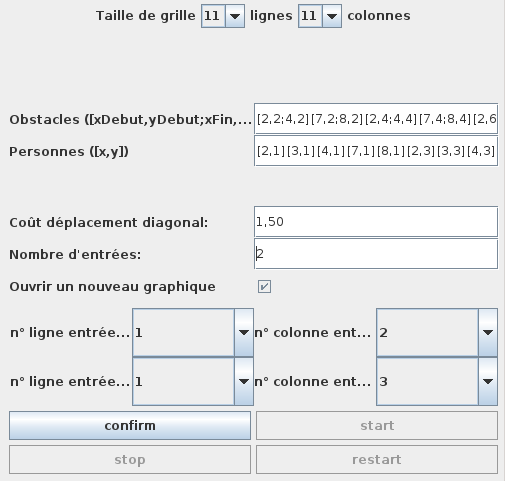
\includegraphics[scale=0.7]{imagesPNG/personnalisation.png}
	\caption{Représentation des distances parcourues}
	\label{fig:distances_parcourues}
	\end{figure}
		
	Une fois cette personnalisation effectuée et validée, la grille est générée, et les fenêtres contenant les diagrammes s'ouvrent en parallèle. L'utilisateur n'a plus qu'à cliqué sur le boutons "Start" pour démarrer la simulation de l'évacuation. Cette dernière continuera jusqu'à ce que l'évacuation soit complète, en mettant à jour les diagrammes en temps réel. Cependant, l'utilisateur a la possibilité de stopper la simulation grâce au bouton "Stop".
		
	\textbf{SCREENSHOT}
		
\chapter{Analyse du projet}
	\section{Compétences acquises}
	Ce projet nous a permis d'asseoir nos compétences dans le développement Java. Cependant, la partie la plus importante a été de mêler nos enseignements en développement aux enseignements plus mathématiques que sont les matières de Sciences de la Décision.\\
	
	En fournissant des mesures exploitables lors de l'implémentation d'un modèle mathématique, il nous a été possible de voir concrètement le lien important qu'il existe en l'informatique et les mathématiques. Il est évident que grâce au mélange de ces deux domaines, ils nous été possible de fournir ``facilement'' et efficacement une simulation précise du fonctionnement du monde réel.
	
	\begin{figure}[!H]
	\centering
	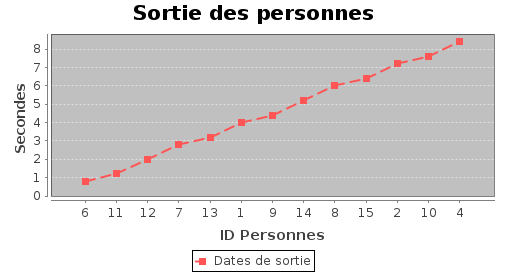
\includegraphics[scale=0.7]{imagesPNG/dateSortie.png}
	\caption{Représentation des dates de sortie}
	\label{fig:date_sortie}
	\end{figure}
	
	\begin{figure}[!H]
	\centering
	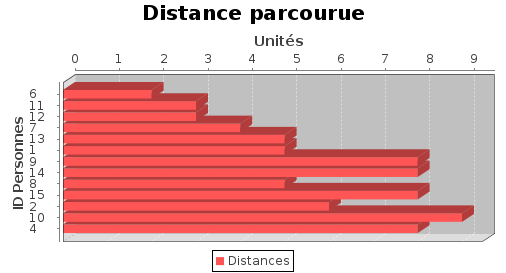
\includegraphics[scale=0.7]{imagesPNG/distanceParcourue.png}
	\caption{Représentation des distances parcourues}
	\label{fig:distances_parcourues}
	\end{figure}
	
	\section{Améliorations possibles}

	\section{Reste à faire}
	
\annexes

\end{document}

